\documentclass[11pt,a4paper]{article}
\usepackage{fontspec}
\setmainfont{Latin Modern Roman}[
  SmallCapsFont={Latin Modern Roman Caps},
  SmallCapsFeatures={Letters=SmallCaps}
]
\setsansfont{Latin Modern Sans}
\setmonofont{Latin Modern Mono}
\usepackage[spanish,es-nodecimaldot]{babel}
\usepackage{geometry}
\geometry{top=2.2cm,bottom=2.2cm,left=2.4cm,right=2.4cm,headheight=15pt}
\usepackage{graphicx}
\usepackage{float}
\usepackage{booktabs}
\usepackage{longtable}
\usepackage{array}
\usepackage{tabularx}
\usepackage{enumitem}
\usepackage{xspace}
\usepackage{xcolor}
\usepackage{hyperref}
\usepackage{fancyhdr}
\usepackage{titlesec}
\usepackage{pdflscape}
\usepackage{microtype}
\usepackage[most]{tcolorbox}

\definecolor{updsblue}{HTML}{0F2742}
\definecolor{accent}{HTML}{2563EB}
\definecolor{lightblue}{HTML}{EAF2FF}
\definecolor{softgray}{HTML}{F6F8FB}
\definecolor{success}{HTML}{166534}
\definecolor{warning}{HTML}{92400E}
\definecolor{danger}{HTML}{991B1B}
\hypersetup{
  colorlinks=true,
  linkcolor=updsblue,
  urlcolor=accent,
  citecolor=updsblue,
  pdftitle={UPDS JUDGE - Informe final},
  pdfauthor={Equipo UPDS JUDGE},
  pdfsubject={Informe académico final del proyecto UPDS JUDGE}
}
\pagestyle{fancy}
\fancyhf{}
\lhead{UPDS JUDGE}
\rhead{Informe final}
\cfoot{\thepage}
\titleformat{\part}[display]{\centering\Huge\bfseries\color{updsblue}}{Fase \thepart}{0.5em}{}
\titleformat{\section}{\Large\bfseries\color{updsblue}}{\thesection.}{0.5em}{}
\titleformat{\subsection}{\large\bfseries\color{accent}}{\thesubsection.}{0.5em}{}
\makeatletter
\renewcommand*\l@subsection{\@dottedtocline{2}{3.8em}{3.5em}}
\makeatother
\setlist[itemize]{topsep=4pt,itemsep=2pt,leftmargin=1.6em}
\setlist[enumerate]{topsep=4pt,itemsep=2pt,leftmargin=1.8em}
\renewcommand{\arraystretch}{1.18}
\setlength{\emergencystretch}{2em}
\newtcolorbox{notebox}[1][]{colback=lightblue,colframe=accent,boxrule=0.7pt,arc=2mm,#1}
\newcommand{\statusimpl}{\textbf{IMPLEMENTADO}\xspace}
\newcommand{\statuslim}{\textbf{IMPLEMENTADO CON LIMITACIONES}\xspace}
\newcommand{\statuspartial}{\textbf{IMPLEMENTADO PARCIALMENTE}\xspace}
\newcommand{\statusno}{\textbf{NO IMPLEMENTADO}\xspace}
\newcommand{\sourceNote}[1]{\par\smallskip{\footnotesize\textit{Fuente: #1}}}
\newcommand{\reportfigure}[4][0.88]{%
  \begin{figure}[H]
    \centering
    \includegraphics[width=#1\textwidth,height=0.72\textheight,keepaspectratio]{#2}
    \caption{#3. Fuente: #4.}
  \end{figure}}

\begin{document}

\hypersetup{pageanchor=false}
\begin{titlepage}
\thispagestyle{empty}
\pagecolor{white}
\centering
\vspace*{0.45cm}
{\Large\bfseries\color{updsblue} UNIVERSIDAD PRIVADA DOMINGO SAVIO\par}
\vspace{0.32cm}
{\color{accent}\rule{0.62\textwidth}{1.1pt}\par}
\vspace{0.55cm}
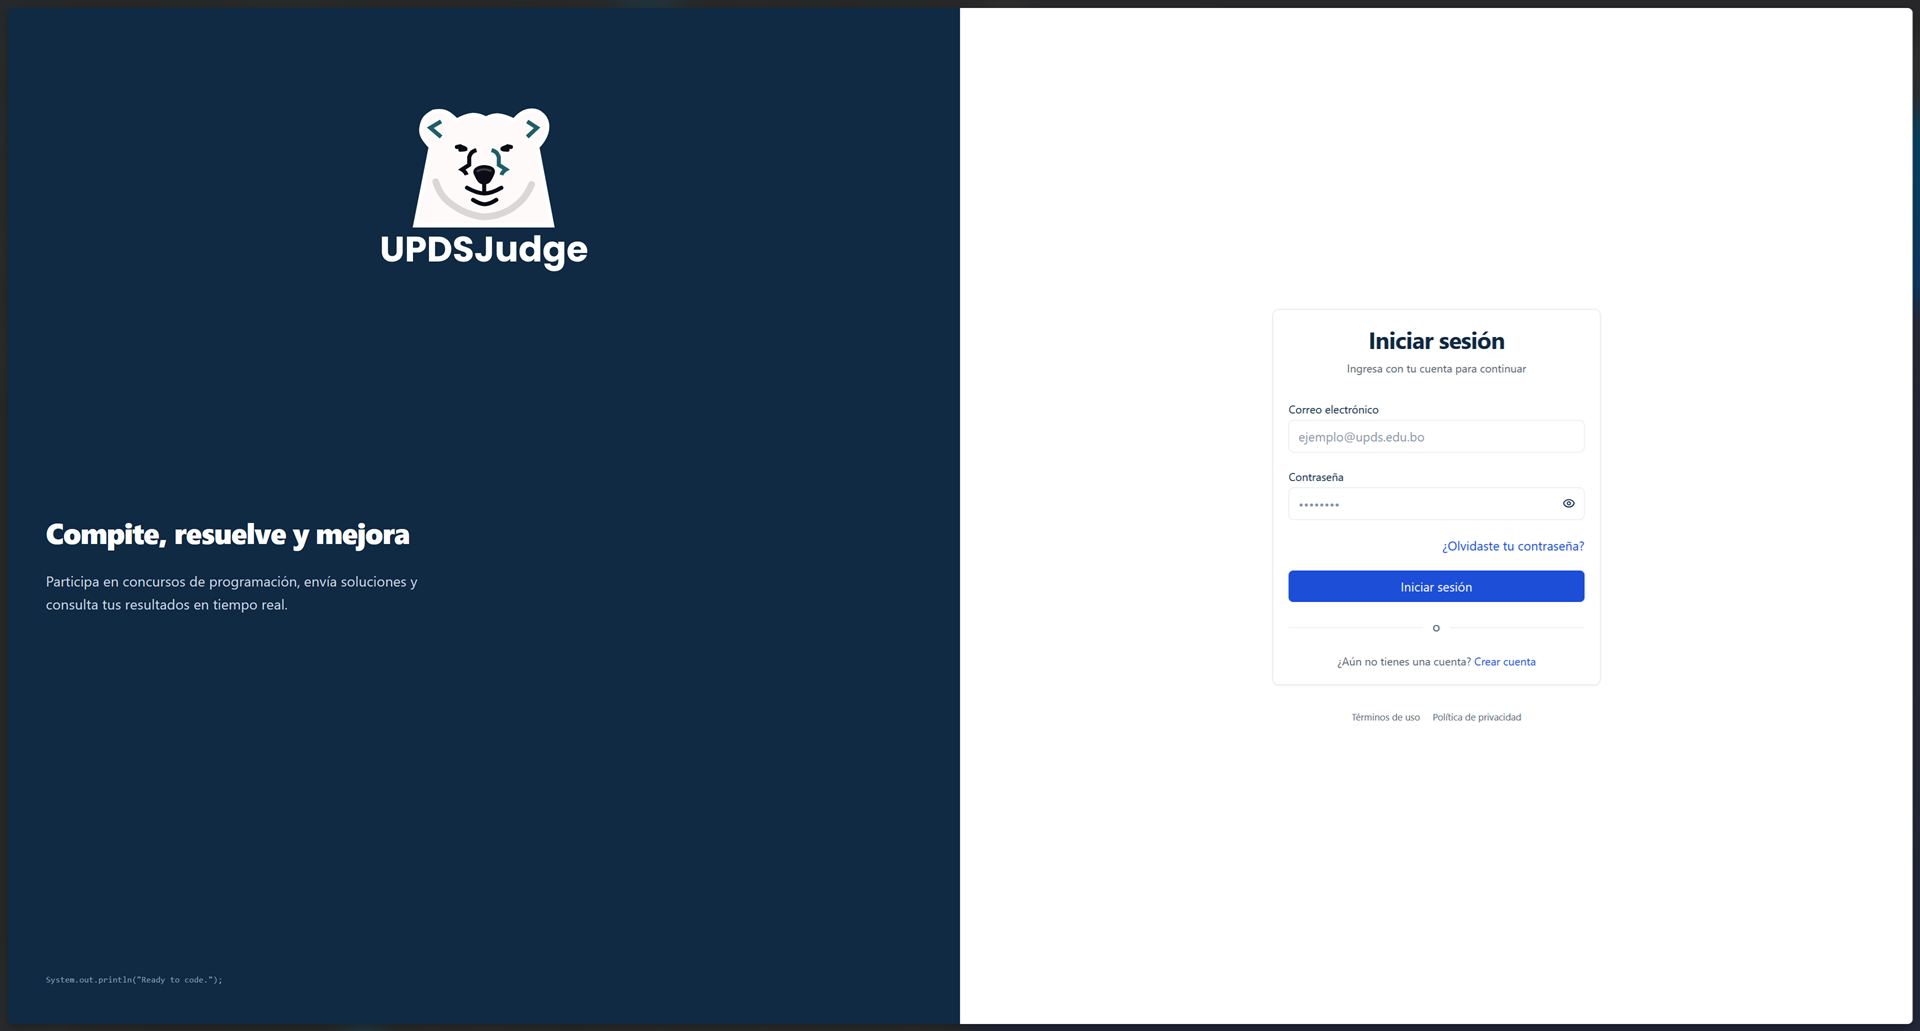
\includegraphics[
  width=3.7cm,
  trim=278bp 561bp 994bp 64bp,
  clip
]{capturas/retrospective-auth-logo.png}
\vspace{0.45cm}

{\large\bfseries\color{updsblue} INFORME FINAL\par}
\vspace{0.32cm}
{\Huge\bfseries\color{updsblue} UPDS JUDGE\par}
\vspace{0.32cm}
{\Large Plataforma web para concursos de programación competitiva\par}
\vspace{0.22cm}
{\large\color{updsblue} Análisis, diseño, implementación y validación\par}
\vspace{0.62cm}

{\large\bfseries\color{updsblue} Integrantes\par}
\vspace{0.22cm}
\begin{minipage}{0.72\textwidth}
\centering
Wilson Yucra Rengifo\\[0.07cm]
Cristhian Joel Amador Gallardo\\[0.07cm]
Arnold Daniel Torrez Zarate\\[0.07cm]
Daniel Javier Aramayo Mancilla\\[0.07cm]
Enny Anaí Lopez Saldaña Beymar\\[0.07cm]
Angelo Vasquez Acha\\[0.07cm]
Alex Saul Fernandez Valdez
\end{minipage}

\vfill
{\color{accent}\rule{0.38\textwidth}{0.8pt}\par}
\vspace{0.28cm}
{\large 29 de julio de 2026\par}
\end{titlepage}
\nopagecolor
\hypersetup{pageanchor=true}
\pagenumbering{roman}

\section*{Revisión histórica}
\addcontentsline{toc}{section}{Revisión histórica}
\begin{table}[H]
\centering
\begin{tabularx}{\textwidth}{>{\bfseries}p{1.7cm}Xp{3.2cm}}
\toprule
Versión & Hito documental & Fecha \\
\midrule
0.1 & Versión inicial del informe con diagnóstico, MVP, backlog, UML y arquitectura propuesta. & Sin fecha documentada \\
0.2 & Reconciliación con la auditoría documental aprobada y el estado vigente del frontend. & 28/07/2026 \\
0.3 & Incorporación de los requerimientos iniciales RF-01 a RF-27 y RNF-01 a RNF-19. & 29/07/2026 \\
0.4 & Incorporación de planificación, matriz RACI y gestión de riesgos. & 29/07/2026 \\
1.0 & Versión final compilada para revisión manual del responsable del proyecto. & 29/07/2026 \\
1.1 & Incorporación de guía de despliegue, entrevista, actores, recursos digitales y README operativo. & 29/07/2026 \\
\bottomrule
\end{tabularx}
\caption{Revisión histórica del informe.}
\label{tab:revision-historica}
\end{table}

\section*{Resumen ejecutivo}
\addcontentsline{toc}{section}{Resumen ejecutivo}
UPDS JUDGE es una plataforma académica para organizar concursos de programación competitiva, administrar identidades y permisos, publicar problemas, recibir soluciones, delegar su evaluación a un juez en línea y presentar veredictos, historial y ranking. El producto final integra un frontend React con contratos HTTP de un backend ASP.NET Core y un motor de evaluación documentado. La descripción de backend, persistencia y juez se basa en la documentación técnica final aprobada por el equipo; dichos componentes y sus contratos se consideran correctos para este informe.

El proyecto entregó los flujos centrales de registro, autenticación, roles, concursos públicos y privados, inscripción, problemas, descarga del conjunto de problemas, envío de soluciones, consulta de resultados, historial, ranking, congelamiento, globos, upsolving y administración. La actualización del historial y del ranking se realiza mediante HTTP y polling; no existe un cliente SignalR o WebSocket conectado en el frontend. La principal desviación funcional es \textbf{RF-02 --- Gestión de perfiles}, cuyo estado final es \statusno. Por la misma ausencia, \textbf{RF-22 --- Participación del usuario} se clasifica como \statuspartial, aun cuando sus restantes subcapacidades fueron entregadas.

El documento integra la especificación de requisitos de software (SRS), la arquitectura, el modelado, la gestión Scrum, la planificación, los riesgos, la validación y una matriz de trazabilidad de 46 requerimientos iniciales. Las propuestas de versiones estables de lenguajes y actualización de datos personales, registradas en la retrospectiva del Sprint 3, permanecen como trabajo futuro no implementado.

\clearpage
\tableofcontents
\clearpage
\listoffigures
\addcontentsline{toc}{section}{Índice de figuras}
\clearpage
\listoftables
\addcontentsline{toc}{section}{Índice de tablas}
\clearpage
\pagenumbering{arabic}

\part{Fundamentos y alcance}

\section{Introducción y objetivos}
\label{sec:introduccion}

\subsection{Propósito}
El propósito de este informe es consolidar, en una estructura académica coherente, la evolución y el resultado final de UPDS JUDGE. Se integran la intención inicial, las historias de usuario, el estado implementado, los hotfixes, las limitaciones y el trabajo futuro, sin confundir planificación histórica con funcionalidad vigente.

\subsection{Antecedentes}
La programación competitiva requiere coordinar participantes, concursos, problemas, lenguajes, envíos, casos de prueba, veredictos y posiciones. La documentación inicial identificó que el uso de herramientas separadas elevaba la carga operativa y dificultaba conservar trazabilidad. El proyecto se planteó como una plataforma web con frontend y backend separados, persistencia en PostgreSQL y un motor especializado de evaluación.

\subsection{Problema identificado}
La comunidad académica necesitaba una plataforma integrada para organizar concursos, evaluar automáticamente las soluciones y publicar resultados oportunos. La fragmentación del proceso producía riesgo de inconsistencias, demora en los veredictos y dificultad para mantener un historial y ranking confiables.

La Figura~\ref{fig:arbol-problemas} sintetiza las causas operativas, técnicas y de gestión que dieron origen al proyecto.
\reportfigure[0.82]{images/arbol-problemas.png}{Árbol de problemas de UPDS JUDGE}{documentación inicial aprobada del proyecto}
\label{fig:arbol-problemas}

\subsection{Alcance}
El alcance incluye identidad y autorización por roles; administración y participación en concursos; importación y configuración de problemas; recepción y evaluación de soluciones; veredictos; historial; ranking; congelamiento; globos; upsolving; y navegación administrativa de Acceso de Usuario. Quedan fuera del producto entregado la gestión editable del perfil, el cliente push en tiempo real, la ampliación contractual del catálogo de lenguajes, la detección de plagio y un editor colaborativo.

\subsection{Objetivo general}
Diseñar e implementar un MVP de UPDS JUDGE que permita administrar concursos de programación, recibir y evaluar soluciones de forma automatizada, consultar veredictos y calcular rankings trazables mediante un frontend React con Vite y un backend ASP.NET Core MVC/Web API separado.

\subsection{Objetivos específicos}
\begin{enumerate}
  \item Implementar autenticación y autorización por roles.
  \item Permitir la creación, edición y consulta de concursos, incluida la importación segura de problemas.
  \item Integrar el flujo de evaluación para C++, Python y C\#.
  \item Conservar un historial de envíos con estado, veredicto, tiempo y memoria.
  \item Calcular ranking, penalización y congelamiento sin incorporar upsolving al resultado oficial.
  \item Proporcionar interfaces consistentes, responsivas y accesibles para usuarios y administradores.
  \item Mantener trazabilidad entre requerimientos, historias, changes, evidencias y resultados.
\end{enumerate}

\subsection{Product Goal}
Centralizar el ciclo de una competencia académica ---desde la configuración hasta el resultado--- para reducir trabajo manual, aplicar reglas uniformes y ofrecer a participantes y organizadores información trazable.

\subsection{Organización del documento}
El informe se organiza en seis fases: fundamentos y alcance; especificación funcional; diseño; gestión ágil; planificación y control; e implementación, validación y cierre. Los anexos reúnen glosario, referencias documentales y orientación sobre evidencias sin duplicar la matriz canónica de trazabilidad.

\section{Toma de requerimientos}

\subsection{Técnicas utilizadas}
La toma y consolidación de requerimientos combinó análisis del problema y de actores, entrevista, revisión de necesidades académicas, historias de usuario, backlog, modelado UML, prototipos visuales documentados, criterios de aceptación, retrospectivas de Sprint y validación documental. Para el cierre se utilizó la auditoría documental aprobada como fuente prioritaria del estado vigente. No se atribuyen al proceso encuestas, talleres ni reuniones no documentadas.

\subsubsection{Entrevista}
La entrevista tuvo como propósito comprender el contexto académico y competitivo, identificar actores y validar necesidades administrativas y de participación. La síntesis autorizada por el responsable relaciona esta técnica con administración de roles, organización y privacidad de concursos, carga de problemas y casos de prueba, participación estudiantil, envíos, ranking y control de resultados. La entrevista contribuyó a identificar y validar estas necesidades; no se afirma que cada requerimiento haya sido pronunciado literalmente en el audio ni se utiliza la entrevista como evidencia de implementación.

El recurso autorizado es \href{https://drive.google.com/file/d/11f3wTCXvLU2kvgIwGbDxx9W_j6ErCma9/view?usp=drivesdk}{Audio de la entrevista de levantamiento de requerimientos}. Para elaborar este informe no fue necesario descargar, analizar ni transcribir el audio; la información funcional utilizada corresponde a la síntesis suministrada por el responsable.

\subsection{Actores}
\begin{description}[style=nextline]
\item[Administrador de Roles --- docente o líder de club.] Usuario con el mayor nivel de privilegios en la gestión de identidades y roles. Consulta y gestiona cuentas dentro de los permisos documentados, asigna el rol Administrador de Concursos a docentes o líderes, administra roles y contribuye a la integridad global. Esto no implica autorización para cualquier operación funcional.
\item[Administrador de Concursos --- docente u organizador.] Responsable de la dimensión académica y competitiva. Crea y edita concursos; configura modalidad pública o privada, información y duración; incorpora el set de problemas en PDF; administra problemas y casos de prueba en ZIP; gestiona participantes y visibilidad de resultados cuando el contrato lo permite; y consulta herramientas administrativas.
\item[Usuario --- estudiante o participante.] Se registra e inicia sesión; consulta e ingresa a concursos según sus reglas; descarga el PDF; consulta problemas; selecciona lenguajes permitidos; envía soluciones; consulta veredictos, historial y ranking; y realiza upsolving cuando corresponde. No dispone de edición de información personal.
\end{description}
Los actores funcionales y los roles de autorización se describen desde las capacidades del sistema. No deben confundirse con roles Scrum ni con responsabilidades de la matriz RACI, que corresponden al trabajo del equipo del proyecto.

\subsection{Stakeholders}
Además de los actores funcionales, son stakeholders el equipo de desarrollo, el evaluador académico y los responsables de operación de backend y juez. El motor de evaluación participa como sistema externo, no como rol humano.

\subsection{Glosario inicial}
Los términos principales se desarrollan en el Anexo~\ref{sec:glosario}. En el contexto funcional, \emph{veredicto} es el resultado normalizado de un envío; \emph{upsolving} es la práctica posterior que no modifica el ranking oficial; y \emph{congelamiento} es el corte temporal que oculta resultados recientes en la vista pública.

\subsection{Supuestos y dependencias}
Se consideran correctos el backend, el juez, los contratos consumidos y los diagramas aprobados. La operación depende de los servicios HTTP, de la persistencia y de la disponibilidad del motor de evaluación. La descripción no implica una nueva auditoría de dichos componentes.

\subsection{Restricciones}
El frontend y el backend permanecen separados; el navegador no ejecuta soluciones ni accede directamente al juez; los casos de prueba son privados; y el catálogo inicial se limita a C++ (\texttt{.cpp}), C\# (\texttt{.cs}) y Python (\texttt{.py}). La propuesta de ampliar versiones o lenguajes no forma parte del producto entregado.

\part{Especificación funcional}

\section{Descripción general del producto}

\subsection{Perspectiva}
UPDS JUDGE es una aplicación web de tipo SPA (Single Page Application) que consume contratos HTTP/JSON. El backend aplica reglas, autorización, persistencia y coordinación con el juez. La Figura~\ref{fig:soluciones} resume la respuesta propuesta al problema inicial.
\reportfigure[0.82]{images/arbol-soluciones.png}{Árbol de soluciones de UPDS JUDGE}{documentación inicial aprobada del proyecto}
\label{fig:soluciones}

\subsection{Características principales}
Las características finales incluyen autenticación y sesión, guards de navegación, layouts por rol, concursos, inscripción pública y privada, problemas, PDF, envíos, veredictos, historial global y contextual, ranking, congelamiento, paginación, globos, edición de concursos y administración de roles.

\subsection{Clases de usuario}
El \textbf{Usuario}, estudiante o participante, opera bajo rutas \texttt{/student} para concursos, problemas, envíos, historial, ranking y upsolving; no cuenta con una pantalla de perfil editable. El \textbf{Administrador de Concursos}, docente u organizador, utiliza rutas de administración y Acceso de Usuario para configurar concursos y consultar sus herramientas. El \textbf{Administrador de Roles}, docente o líder de club, utiliza \texttt{/admin/roles} para consultar usuarios y administrar asignaciones permitidas. Los guards frontend controlan navegación y experiencia de usuario, mientras la autorización definitiva corresponde al backend.

\subsection{Interfaces externas}
Las interfaces externas principales son la API HTTP del backend, la persistencia PostgreSQL y el motor de evaluación. El frontend centraliza endpoints, transporte autenticado y tipos contractuales. La actualización del ranking usa polling de diez segundos; el historial se vuelve a consultar tras un envío.

\subsection{Interfaces de usuario}
La interfaz dispone de plantillas de autenticación, \texttt{UserLayout}, \texttt{AdminLayout}, sidebar administrativo, encabezado contextual de concurso, formularios, tablas, filtros, paginación, mensajes de carga/vacío/error y componentes de veredictos y globos.

\section{Requerimientos}
\label{sec:requerimientos}

\subsection{Requerimientos funcionales iniciales}
La Tabla~\ref{tab:rf-iniciales} conserva los 27 requerimientos iniciales sin reformularlos para acomodarlos al resultado final.

\begin{longtable}{>{\bfseries}p{1.4cm}p{12.8cm}}
\caption{Requerimientos funcionales iniciales.}\label{tab:rf-iniciales}\\
\toprule
ID & Requerimiento inicial \\
\midrule
\endfirsthead
\toprule
ID & Requerimiento inicial \\
\midrule
\endhead
RF-01 & Registro e inicio de sesión. \\
RF-02 & Gestión de perfiles: visualizar y editar información básica del perfil del usuario. \\
RF-03 & Listado de concursos. \\
RF-04 & Visualización del concurso. \\
RF-05 & Participación en concursos. \\
RF-06 & Listado de problemas. \\
RF-07 & Descarga del conjunto de problemas. \\
RF-08 & Envío de soluciones. \\
RF-09 & Selección de lenguaje. \\
RF-10 & Evaluación automática. \\
RF-11 & Verificación de casos de prueba. \\
RF-12 & Resultado del envío. \\
RF-13 & Historial de envíos. \\
RF-14 & Ranking del concurso. \\
RF-15 & Administración de problemas. \\
RF-16 & Administración de casos de prueba. \\
RF-17 & Gestión de usuarios. \\
RF-18 & Upsolving. \\
RF-19 & Consulta de resultados. \\
RF-20 & Administración de roles. \\
RF-21 & Administración de concursos. \\
RF-22 & Participación del usuario. \\
RF-23 & Control del estado del concurso. \\
RF-24 & Acceso a concursos. \\
RF-25 & Validación de archivos. \\
RF-26 & Consulta del estado de los envíos. \\
RF-27 & Gestión de participantes. \\
\bottomrule
\end{longtable}

\subsection{Requerimientos no funcionales iniciales}
\begin{longtable}{>{\bfseries}p{1.6cm}p{12.6cm}}
\caption{Requerimientos no funcionales iniciales.}\label{tab:rnf-iniciales}\\
\toprule
ID & Requerimiento inicial \\
\midrule
\endfirsthead
\toprule
ID & Requerimiento inicial \\
\midrule
\endhead
RNF-01 & Rendimiento. \\
RNF-02 & Escalabilidad. \\
RNF-03 & Disponibilidad. \\
RNF-04 & Seguridad. \\
RNF-05 & Integridad de la evaluación. \\
RNF-06 & Aislamiento de ejecución. \\
RNF-07 & Compatibilidad. \\
RNF-08 & Usabilidad. \\
RNF-09 & Mantenibilidad. \\
RNF-10 & Portabilidad. \\
RNF-11 & Persistencia. \\
RNF-12 & Disponibilidad del motor de evaluación. \\
RNF-13 & Auditoría. \\
RNF-14 & Extensibilidad. \\
RNF-15 & Concurrencia. \\
RNF-16 & Stack tecnológico backend. \\
RNF-17 & Stack tecnológico frontend. \\
RNF-18 & Gestión de base de datos. \\
RNF-19 & Arquitectura de evaluación. \\
\bottomrule
\end{longtable}

\subsection{Estado final de cumplimiento}
El resultado general confirma la entrega del flujo principal, con limitaciones explícitas en actualización push, mediciones operativas y disponibilidad de dependencias externas. Los estados utilizados son \statusimpl, \statuslim, \statuspartial y \statusno. El detalle canónico aparece en la matriz de la Sección~\ref{sec:matriz}.

\subsection{Desviaciones}
Las desviaciones principales son la ausencia de gestión editable del perfil y la falta de push en tiempo real desde el frontend. La primera afecta RF-02 y una subcapacidad de RF-22; la segunda limita RF-12 y RF-26 sin eliminar la consulta funcional por HTTP. Las métricas de rendimiento, disponibilidad y concurrencia no se presentan como garantías cuantificadas si la documentación no registra una medición final.

\subsection{Gestión de perfiles no implementada}
\label{sec:rf02}
\textbf{RF-02 --- Gestión de perfiles. Estado final: NO IMPLEMENTADO.} El requerimiento pedía visualizar y editar la información básica del perfil del usuario. El producto entregado no contiene pantalla editable de perfil, página de configuración personal, formulario de actualización de datos, flujo de guardado ni actualización de sesión derivada de una edición del perfil. La retrospectiva del Sprint 3 registró la actualización de datos personales como propuesta futura, no implementada y pendiente de priorización.

\subsection{Desglose de RF-22}
La Tabla~\ref{tab:rf22} explica por qué el estado global de RF-22 es parcial.
\begin{table}[H]
\centering
\begin{tabularx}{\textwidth}{p{1.4cm}Xp{4.5cm}}
\toprule
ID & Subcapacidad & Estado final \\
\midrule
RF-22.a & Consultar concursos & IMPLEMENTADO \\
RF-22.b & Visualizar un concurso & IMPLEMENTADO \\
RF-22.c & Descargar el PDF & IMPLEMENTADO \\
RF-22.d & Enviar soluciones & IMPLEMENTADO \\
RF-22.e & Consultar estados de envíos & IMPLEMENTADO CON LIMITACIONES \\
RF-22.f & Consultar el ranking & IMPLEMENTADO \\
RF-22.g & Consultar historial de envíos & IMPLEMENTADO \\
RF-22.h & Editar información del perfil & NO IMPLEMENTADO \\
\bottomrule
\end{tabularx}
\caption{Desglose funcional de RF-22.}
\label{tab:rf22}
\end{table}
Por tanto, \textbf{RF-22 --- Participación del usuario} tiene estado global \statuspartial.

\subsection{Matriz de trazabilidad}
\label{sec:matriz}
La matriz completa se presenta una sola vez. La evidencia combina la auditoría documental, las historias reconciliadas, los changes y hotfixes, las retrospectivas, los diagramas y los contratos consumidos. Para backend y juez se aplica la suposición aprobada de corrección.

\begin{landscape}
\begingroup
\setlength{\tabcolsep}{3pt}
\footnotesize
\begin{longtable}{>{\bfseries}p{1.25cm}p{4.0cm}p{1.15cm}p{3.35cm}p{4.5cm}p{4.0cm}p{5.1cm}}
\caption{Matriz canónica de trazabilidad de requerimientos iniciales.}\label{tab:trazabilidad}\\
\toprule
ID & Requerimiento inicial & Tipo & Estado final & Evidencia documental & Historia o change relacionado & Observaciones \\
\midrule
\endfirsthead
\multicolumn{7}{l}{\textit{Continuación de la Tabla~\ref{tab:trazabilidad}}}\\
\toprule
ID & Requerimiento inicial & Tipo & Estado final & Evidencia documental & Historia o change relacionado & Observaciones \\
\midrule
\endhead
\bottomrule
\endfoot
RF-01 & Registro e inicio de sesión & RF & IMPLEMENTADO & Auditoría: rutas \texttt{/register}, \texttt{/login}, sesión y guards & UJ-05, UJ-06 & Registro, token, identidad y cierre de sesión integrados. \\
RF-02 & Gestión de perfiles & RF & NO IMPLEMENTADO & Auditoría y retrospectiva Sprint 3 & Sin historia implementada & No existe pantalla, formulario, servicio ni guardado de perfil editable. \\
RF-03 & Listado de concursos & RF & IMPLEMENTADO & Dashboard de usuario, filtros y paginación & UJ-11 & Concursos próximos, activos y finalizados. \\
RF-04 & Visualización del concurso & RF & IMPLEMENTADO & Rutas contextuales y \texttt{ContestContextHeader} & UJ-11, UJ-13 & Contexto reutilizado para problemas, envíos y ranking. \\
RF-05 & Participación en concursos & RF & IMPLEMENTADO & Política de acceso y endpoint de inscripción & UJ-12 & Incluye públicos y privados, incluso privado finalizado según contrato aprobado. \\
RF-06 & Listado de problemas & RF & IMPLEMENTADO & Feature \texttt{problems} y dashboard contractual & UJ-13 & Incisos, títulos, límites y estado personal. \\
RF-07 & Descarga del conjunto de problemas & RF & IMPLEMENTADO & Botón de PDF documentado y ruta contextual & UJ-13 & Abre el recurso configurado sin bloquear el resto de la pantalla. \\
RF-08 & Envío de soluciones & RF & IMPLEMENTADO & Formulario, editor, carga y POST de envíos & UJ-14 & El código se transmite como texto; no se ejecuta en el navegador. \\
RF-09 & Selección de lenguaje & RF & IMPLEMENTADO & Selector C++ 17, Python 3 y C\# & UJ-14 & Catálogo final no se presenta como ampliado. \\
RF-10 & Evaluación automática & RF & IMPLEMENTADO & Arquitectura y contratos de evaluación aprobados & UJ-14, UJ-15 & Backend y juez se consideran correctos. \\
RF-11 & Verificación de casos de prueba & RF & IMPLEMENTADO & Modelado de casos privados y evaluación & UJ-09, UJ-10, UJ-15 & Casos protegidos y coordinados por backend/juez. \\
RF-12 & Resultado del envío & RF & IMPLEMENTADO CON LIMITACIONES & Historial y \texttt{VerdictBadge} por HTTP & UJ-15 & Resultado visible; no existe push SignalR/WebSocket conectado. \\
RF-13 & Historial de envíos & RF & IMPLEMENTADO & Historial global y contextual, filtros y paginación & UJ-20 & Vistas de usuario y Acceso de Usuario. \\
RF-14 & Ranking del concurso & RF & IMPLEMENTADO & Ranking contractual, polling, paginación y hotfix & UJ-18; fix de regresión UJ-18 & Frontend conserva puestos y penalización del backend. \\
RF-15 & Administración de problemas & RF & IMPLEMENTADO & Creación/edición de concurso y lista de problemas & UJ-08, UJ-09, UJ-10, UJ-19 & Configuración de inciso, límites, memoria y globos. \\
RF-16 & Administración de casos de prueba & RF & IMPLEMENTADO & Importación ZIP y modelo de almacenamiento privado & UJ-09, UJ-10 & Validación y persistencia coordinadas por backend aprobado. \\
RF-17 & Gestión de usuarios & RF & IMPLEMENTADO & Consulta, búsqueda y roles de usuarios & UJ-07 & Capacidad del Administrador de Roles, acotada a permisos; no equivale a perfil personal. \\
RF-18 & Upsolving & RF & IMPLEMENTADO & Backlog, contratos y ranking que excluye práctica & UJ-16, UJ-18 & Los envíos posteriores no alteran el ranking oficial. \\
RF-19 & Consulta de resultados & RF & IMPLEMENTADO & Envíos contextuales e historial global & UJ-15, UJ-20 & Veredictos, tiempo y memoria cuando están disponibles. \\
RF-20 & Administración de roles & RF & IMPLEMENTADO & Ruta \texttt{/admin/roles}, búsqueda, asignación y remoción & UJ-07 & Administrador de Roles: docente o líder de club, dentro de permisos definidos. \\
RF-21 & Administración de concursos & RF & IMPLEMENTADO & Listado, filtros, resumen, creación y edición & UJ-08, UJ-09, UJ-19 & Administrador de Concursos: docente u organizador; incluye ZIP, congelamiento y globos. \\
RF-22 & Participación del usuario & RF & IMPLEMENTADO PARCIALMENTE & Auditoría, UJ-11 a UJ-20 y Tabla~\ref{tab:rf22} & UJ-11--UJ-20 & Usuario estudiante o participante; todas las subcapacidades principales salvo edición de perfil. \\
RF-23 & Control del estado del concurso & RF & IMPLEMENTADO & Fechas, duración, estados y congelamiento & UJ-08, UJ-11, UJ-19 & El backend es fuente de verdad del estado. \\
RF-24 & Acceso a concursos & RF & IMPLEMENTADO & Guards, política de acceso e inscripción & UJ-11, UJ-12 & Acceso por sesión, rol, modalidad y participación. \\
RF-25 & Validación de archivos & RF & IMPLEMENTADO & ZIP, extensiones \texttt{.cpp/.py/.cs} y límite de tamaño & UJ-09, UJ-14, UJ-19 & Validación cliente y servidor; casos permanecen privados. \\
RF-26 & Consulta del estado de los envíos & RF & IMPLEMENTADO CON LIMITACIONES & Refetch HTTP, botón Actualizar e historial & UJ-15, UJ-20 & Sin cliente push en tiempo real. \\
RF-27 & Gestión de participantes & RF & IMPLEMENTADO & Inscripción, participación única y ranking & UJ-12, UJ-18 & Administración y participación según permisos; contratos externos asumidos correctos. \\
RNF-01 & Rendimiento & RNF & IMPLEMENTADO CON LIMITACIONES & Polling acotado, paginación y consultas por dominio & UJ-18, UJ-20 & No se documenta una garantía cuantitativa final de carga. \\
RNF-02 & Escalabilidad & RNF & IMPLEMENTADO CON LIMITACIONES & Separación frontend/backend, servicios y paginación & Arquitectura aprobada & Arquitectura escalable; capacidad no medida en este cierre. \\
RNF-03 & Disponibilidad & RNF & IMPLEMENTADO CON LIMITACIONES & Recuperación HTTP y manejo de errores & UJ-15 & Depende de API, base de datos y juez. \\
RNF-04 & Seguridad & RNF & IMPLEMENTADO & JWT, roles, guards, casos privados y validación & UJ-05--UJ-09 & La autorización definitiva reside en backend. \\
RNF-05 & Integridad de la evaluación & RNF & IMPLEMENTADO & Persistencia de envíos, veredictos y resultados por caso & UJ-14, UJ-15 & Backend y juez aprobados como fuente de verdad. \\
RNF-06 & Aislamiento de ejecución & RNF & IMPLEMENTADO & Juez externo y navegador sin ejecución de código & Arquitectura de evaluación & El frontend nunca ejecuta soluciones. \\
RNF-07 & Compatibilidad & RNF & IMPLEMENTADO & SPA web y catálogo C++, Python, C\# & UJ-14 & No implica ampliación futura de lenguajes. \\
RNF-08 & Usabilidad & RNF & IMPLEMENTADO & Responsive, estados, feedback, filtros y accesibilidad & Historias reconciliadas & Layouts y componentes consistentes por rol. \\
RNF-09 & Mantenibilidad & RNF & IMPLEMENTADO & Organización por features, tipos, mappers y tests & Changes de Sprints 1--3 & Contratos y componentes compartidos reducen duplicación. \\
RNF-10 & Portabilidad & RNF & IMPLEMENTADO CON LIMITACIONES & Cliente web y separación por servicios & Sprint 0; arquitectura aprobada & La documentación no registra una matriz final de plataformas. \\
RNF-11 & Persistencia & RNF & IMPLEMENTADO & PostgreSQL/EF Core y contratos de historial & Arquitectura de datos & Se asume correcta la implementación aprobada. \\
RNF-12 & Disponibilidad del motor de evaluación & RNF & IMPLEMENTADO CON LIMITACIONES & Manejo de 503 y recuperación de estado & UJ-15 & Dependencia externa operativa, sin SLA documentado. \\
RNF-13 & Auditoría & RNF & IMPLEMENTADO & Historial de envíos y auditoría de roles documentada & UJ-07, UJ-20 & Registra acciones y resultados relevantes. \\
RNF-14 & Extensibilidad & RNF & IMPLEMENTADO & Features, servicios, catálogo y adaptadores & Arquitectura aprobada & Extensibilidad arquitectónica no equivale a haber ampliado lenguajes. \\
RNF-15 & Concurrencia & RNF & IMPLEMENTADO CON LIMITACIONES & Evaluación externa, estados, polling y consultas & UJ-15, UJ-18 & No se consigna prueba de carga final. \\
RNF-16 & Stack tecnológico backend & RNF & IMPLEMENTADO & ASP.NET Core MVC/Web API, EF Core & Documentación técnica aprobada & Backend asumido correcto; no fue reauditado. \\
RNF-17 & Stack tecnológico frontend & RNF & IMPLEMENTADO & React, TypeScript, Vite, Tailwind CSS & README y \texttt{package.json} & Stack verificado en el repositorio frontend. \\
RNF-18 & Gestión de base de datos & RNF & IMPLEMENTADO & PostgreSQL, Identity y modelo relacional & Arquitectura de datos & Persistencia descrita desde documentación aprobada. \\
RNF-19 & Arquitectura de evaluación & RNF & IMPLEMENTADO & Backend encapsula juez, casos y resultados & Diagramas y contratos & El navegador no accede al juez ni a casos privados. \\
\end{longtable}
\normalsize
\endgroup
\end{landscape}

\section{Casos de uso y modelado funcional}

\subsection{Diagrama general}
La Figura~\ref{fig:casos-uso} presenta los casos de uso aprobados y su relación con los actores.
\reportfigure[0.86]{images/diagrama-casos-uso.png}{Diagrama general de casos de uso}{fuente PlantUML aprobada del proyecto}
\label{fig:casos-uso}

\subsection{Casos principales}
El Administrador de Roles consulta usuarios y gestiona asignaciones autorizadas; el Administrador de Concursos crea o edita concursos, configura privacidad y duración, incorpora PDF y ZIP, administra problemas y consulta herramientas del concurso; y el Usuario se registra, inicia sesión, se inscribe, consulta problemas, descarga el PDF, envía soluciones y revisa veredictos, historial, ranking y upsolving. Ningún caso de uso entregado permite editar el perfil personal.

\subsection{Flujos básicos y alternativos}
El flujo competitivo básico es autenticación, acceso al concurso, selección de problema y lenguaje, envío, evaluación y consulta del resultado. Entre los flujos alternativos se encuentran contraseña incorrecta, concurso no accesible, archivo inválido, juez temporalmente no disponible, payload contractual inválido y ranking congelado.

\subsection{Relación entre requerimientos e historias}
Las historias UJ-05 a UJ-07 cubren identidad; UJ-08 a UJ-10, administración; UJ-11 a UJ-13, participación; UJ-14 a UJ-16, evaluación; y UJ-18 a UJ-20, ranking e historial. El identificador UJ-17 no existe en la fuente original y no fue inventado.

\part{Diseño de la solución}

\section{Arquitectura}

\subsection{Visión general}
La arquitectura separa la SPA, la API, la persistencia y el motor de evaluación. La Figura~\ref{fig:arquitectura} muestra los componentes y sus dependencias aprobadas.
\reportfigure[0.9]{images/arquitectura-componentes.png}{Arquitectura de componentes de UPDS JUDGE}{fuente PlantUML aprobada del proyecto}
\label{fig:arquitectura}

\subsection{Arquitectura frontend}
El frontend se organiza por features de autenticación, concursos, problemas, envíos, historial, ranking y administración. React Router compone rutas públicas y protegidas; \texttt{UserLayout} y \texttt{AdminLayout} delimitan experiencias; TanStack Query coordina consultas y polling; el cliente HTTP incorpora la sesión; y los tipos generados reflejan el contrato consumido.

\subsection{Backend}
El backend documentado utiliza ASP.NET Core MVC/Web API, servicios de aplicación, Entity Framework Core e Identity. Expone contratos HTTP/JSON para autenticación, roles, concursos, participantes, envíos y ranking. Esta descripción se basa en la documentación técnica final aprobada por el equipo; no se realizó una auditoría adicional.

\subsection{Motor de evaluación}
El juez compila y ejecuta soluciones bajo límites de tiempo y memoria, normaliza estados y devuelve métricas. El backend encapsula sus credenciales y coordina la persistencia. El frontend recibe únicamente el contrato de resultados.

\subsection{Comunicación entre componentes}
La Figura~\ref{fig:secuencia-envio} representa el flujo de envío, evaluación y persistencia. El frontend crea la solicitud, el backend valida identidad y reglas, el servicio de evaluación coordina el juez y la base de datos conserva el resultado.
\reportfigure[0.92]{images/secuencia-envio-solucion.png}{Secuencia de envío y evaluación de una solución}{fuente PlantUML aprobada del proyecto}
\label{fig:secuencia-envio}

\subsection{Seguridad y roles}
JWT identifica la sesión y los roles; los guards evitan navegación incompatible; y el backend valida autorización. El Administrador de Roles no recibe autorización funcional irrestricta por su denominación; el Administrador de Concursos se limita a las capacidades administrativas documentadas; y el Usuario accede a funciones competitivas según inscripción, modalidad y estado del concurso. Los casos de prueba, código y credenciales no se exponen al navegador. La extracción ZIP requiere límites y prevención de rutas maliciosas.

\section{Modelado}

\subsection{Diagrama de clases}
La Figura~\ref{fig:clases} relaciona Usuario, Rol, Concurso, Participación, Problema, Caso de Prueba, Lenguaje, Envío y Resultado.
\reportfigure[0.9]{images/diagrama-clases-persistencia.png}{Diagrama de clases de persistencia}{fuente PlantUML aprobada del proyecto}
\label{fig:clases}

\subsection{Modelo de contexto}
La Figura~\ref{fig:contexto} distingue frontend, backend, persistencia y juez. Cualquier conexión de tiempo real representada se interpreta como integración prevista, porque el frontend final no contiene un cliente SignalR o WebSocket conectado.
\reportfigure[0.86]{images/modelo-contexto.png}{Modelo de contexto técnico y actores}{fuente PlantUML aprobada del proyecto}
\label{fig:contexto}

\subsection{Diagramas de secuencia o actividad}
Además de la secuencia de envío, la Figura~\ref{fig:secuencia-zip} documenta la importación del ZIP con validación previa, tratamiento transaccional y almacenamiento privado.
\reportfigure[0.9]{images/secuencia-importacion-zip.png}{Secuencia de importación de problemas y casos desde ZIP}{fuente PlantUML aprobada del proyecto}
\label{fig:secuencia-zip}

\subsection{Modelo de datos}
La Figura~\ref{fig:modelo-relacional} presenta el modelo relacional aprobado. Identity conserva credenciales y roles; concursos y participaciones delimitan acceso; problemas y casos representan la competencia; y envíos y resultados sostienen trazabilidad y ranking.
\reportfigure[0.84]{images/modelo-relacional.png}{Modelo relacional de UPDS JUDGE}{fuente PlantUML aprobada del proyecto}
\label{fig:modelo-relacional}

\subsection{Diccionario de datos o referencia}
Las entidades principales son Concurso, ParticipaciónConcurso, Problema, CasoPrueba, Lenguaje, Envío y ResultadoCaso. El diccionario detallado permanece en la arquitectura de datos aprobada; este informe evita duplicarlo y conserva la referencia documental en la bibliografía.

\part{Gestión ágil}

\section{Metodología Scrum}

\subsection{Organización del equipo}
El equipo trabajó de manera incremental con backlog, historias, criterios, changes, revisiones y retrospectivas. La responsabilidad funcional del producto permaneció separada de la coordinación del equipo y de las asignaciones de ejecución.

\subsection{Roles Scrum}
La documentación registra coordinación del squad, revisión, evidencias, pruebas, backend y assets. No existe evidencia suficiente para reinterpretar esas responsabilidades como una designación formal adicional; por ello se conservan únicamente las funciones documentadas.

\subsection{Matriz RACI}
La Figura~\ref{fig:matriz-raci} muestra la asignación de responsabilidades utilizada por el equipo. Se interpreta como instrumento de coordinación: identifica participación y responsabilidad por actividad sin confundirse con los permisos del sistema. No se expanden abreviaturas o identidades que no estén definidas en la fuente.

\clearpage
\begin{landscape}
\begin{figure}[H]
\centering
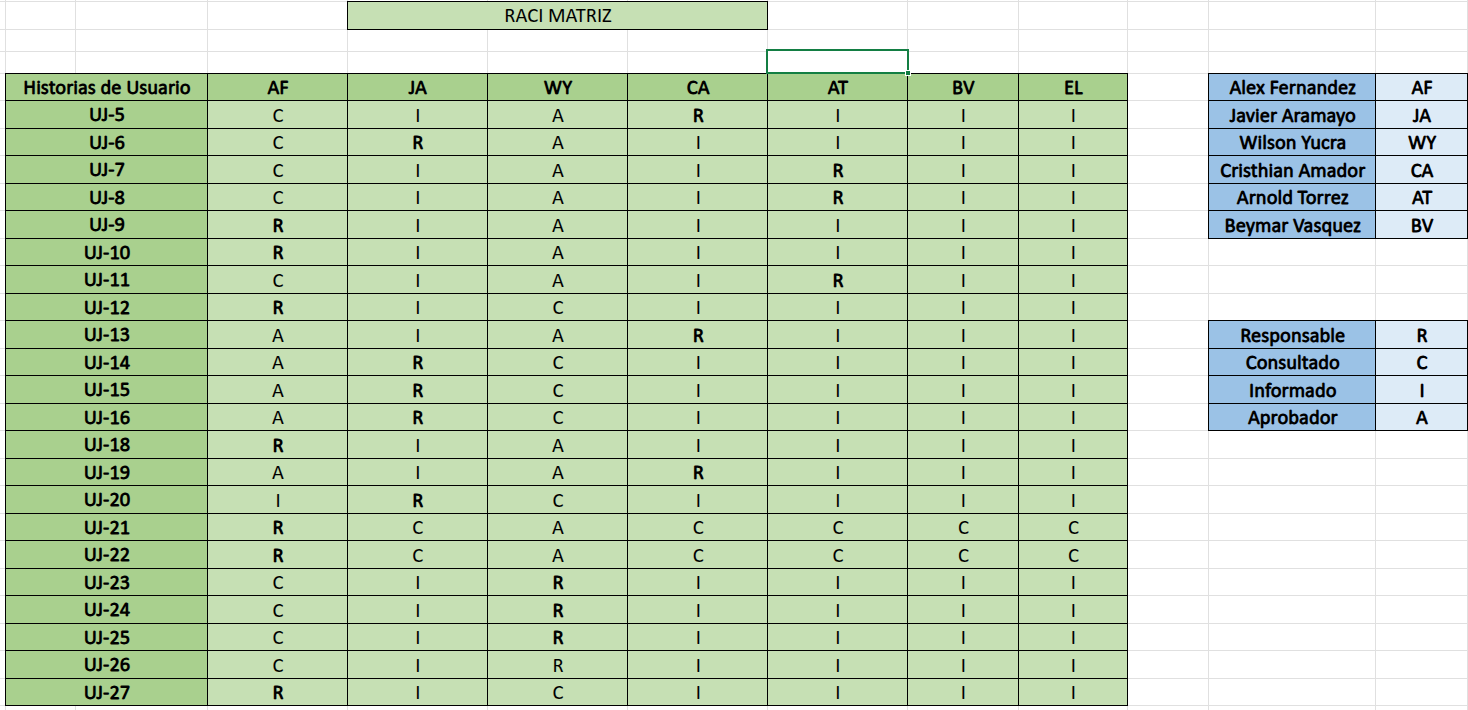
\includegraphics[width=0.94\linewidth,height=0.73\textheight,keepaspectratio]{images/RaciMatriz.png}
\caption{Matriz RACI del proyecto. Fuente: elaboración del equipo del proyecto.}
\label{fig:matriz-raci}
\end{figure}
\end{landscape}
\clearpage

\subsection{Product Backlog}
El backlog contiene 15 historias y cinco épicas. La Tabla~\ref{tab:backlog-resumen} resume su distribución sin repetir criterios completos.
\begingroup
\setlength{\tabcolsep}{3pt}
\begin{longtable}{>{\bfseries}p{1.4cm}p{6.2cm}p{1.5cm}p{2.6cm}p{3.2cm}}
\caption{Resumen del Product Backlog y estado final.}\label{tab:backlog-resumen}\\
\toprule
ID & Resumen & Sprint & Estado final & Requerimientos relacionados \\
\midrule
\endfirsthead
\toprule
ID & Resumen & Sprint & Estado final & Requerimientos relacionados \\
\midrule
\endhead
UJ-05 & Registro de usuario & 1 & Implementado & RF-01, RNF-04 \\
UJ-06 & Inicio de sesión y token con roles & 1 & Implementado & RF-01, RF-24 \\
UJ-07 & Asignar y revocar roles & 3 & Implementado & RF-17, RF-20 \\
UJ-08 & Crear y administrar concurso & 1 & Implementado & RF-21, RF-23 \\
UJ-09 & Importar paquete ZIP & 1 & Implementado & RF-15, RF-16, RF-25 \\
UJ-10 & Configurar problemas & 2 & Implementado & RF-15, RF-16 \\
UJ-11 & Listar concursos por estado & 2 & Implementado & RF-03, RF-04 \\
UJ-12 & Inscribirse a concursos & 2 & Implementado & RF-05, RF-24, RF-27 \\
UJ-13 & Consultar problemas y PDF & 2 & Implementado & RF-06, RF-07 \\
UJ-14 & Enviar solución & 2 & Implementado & RF-08, RF-09, RF-25 \\
UJ-15 & Recibir y consultar veredicto & 2 & Con limitaciones & RF-12, RF-19, RF-26 \\
UJ-16 & Practicar mediante upsolving & 3 & Implementado & RF-18 \\
UJ-18 & Consultar ranking & 3 & Implementado & RF-14 \\
UJ-19 & Configurar congelamiento & 3 & Implementado & RF-21, RF-23 \\
UJ-20 & Consultar historial global & 3 & Implementado & RF-13, RF-19 \\
\bottomrule
\end{longtable}
\endgroup

\subsection{Product Goal}
El Product Goal fue disponer de un flujo integrado y trazable de concursos de programación, desde identidad y configuración hasta evaluación y ranking. Su logro se evalúa en la Sección~\ref{sec:resultados}.

\subsection{Sprint Backlogs y Sprint Goals}
Sprint 0 preparó fundaciones; Sprint 1 buscó habilitar login y creación de concursos con ZIP; Sprint 2 concentró participación y juez; y Sprint 3 cerró ranking, congelamiento, historial y roles. La asignación se conserva según el plan documentado.

\section{Ejecución de Sprints}

\subsection{Sprint 0}
El Sprint 0 definió repositorios, ramas, estructura React/Vite/TypeScript, backend ASP.NET Core, persistencia, contratos, CORS, variables y componentes base. Su resultado fue una fábrica de software y documentación inicial para ejecutar historias incrementales.

\subsection{Sprint 1}
El Sprint 1 cubrió autenticación, shell, administración de concursos, creación e importación ZIP. La retrospectiva destacó la necesidad de contratos estables, boundaries de features, componentes reutilizables y validación reproducible. UJ-11 permanecía futura en ese momento, pero fue implementada posteriormente.

\subsection{Sprint 2}
El Sprint 2 consolidó participación, concursos privados, problemas, envíos y contexto reutilizable. Sus acuerdos posteriores incorporaron Acceso de Usuario bajo \texttt{AdminLayout}, la política de privado finalizado, remediación de dependencias y \texttt{ContestContextHeader}. La retrospectiva conserva la diferencia entre acuerdo histórico e implementación posterior.

\subsection{Sprint 3}
El Sprint 3 integró roles, acceso administrativo de usuario, edición de concursos, congelamiento, colores de globos, ranking, polling, paginación, historial y hotfixes. También registró dos propuestas futuras: versiones estables de lenguajes y actualización de datos personales.

\subsection{Sprint Reviews}
Las reviews se documentaron mediante criterios de aceptación, changes, pruebas y confirmaciones manuales existentes. Cuando una ceremonia no dispone de acta específica, este informe no inventa asistentes, decisiones ni fechas.

\subsection{Retrospectivas}
Las retrospectivas aplicaron la técnica Starfish y distinguieron prácticas a mantener, reducir, ampliar, detener e iniciar. Los aprendizajes centrales fueron validar contratos antes de integrar, mantener layouts como contenedores, usar datos contractuales y complementar pruebas unitarias con router y requests reales.

\subsection{Acciones futuras no implementadas}
\begin{notebox}
\textbf{Versiones estables de lenguajes: propuesta no implementada.} El catálogo actual no demuestra una ampliación contractual ni nuevos runtimes.\\[0.25cm]
\textbf{Configuración y actualización de datos personales: propuesta no implementada.} No existe ruta, pantalla, formulario o servicio de perfil editable.
\end{notebox}

\part{Planificación y control}

\section{Planificación temporal}

\subsection{Gantt general por Sprint}
La Figura~\ref{fig:gantt-sprints} representa la secuencia general de Sprints y respalda el seguimiento de las fases de fundación, administración, participación y cierre. La lectura horizontal permite relacionar duración relativa y orden de ejecución sin introducir fechas adicionales a las consignadas en la fuente.

\clearpage
\begin{landscape}
\begin{figure}[H]
\centering

\includegraphics[width=0.96\linewidth,height=0.68\textheight,keepaspectratio]{\detokenize{images/Captura de pantalla 2026-07-28 204707.png}}
\caption{Diagrama de Gantt general por Sprint. Fuente: elaboración del equipo del proyecto.}
\label{fig:gantt-sprints}
\end{figure}
\end{landscape}
\clearpage

\subsection{Gantt de historias de usuario}
La Figura~\ref{fig:gantt-historias} distribuye las historias dentro del calendario del proyecto. Su función es evidenciar dependencias y concentración de trabajo, especialmente entre identidad, concursos, juez y ranking.

\clearpage
\begin{landscape}
\begin{figure}[H]
\centering

\includegraphics[width=0.95\linewidth,height=0.72\textheight,keepaspectratio]{\detokenize{images/Captura de pantalla 2026-07-28 204726.png}}
\caption{Distribución temporal de historias de usuario. Fuente: elaboración del equipo del proyecto.}
\label{fig:gantt-historias}
\end{figure}
\end{landscape}
\clearpage

\subsection{Hitos y entregables}
Los hitos fueron: fundaciones y contratos; autenticación y administración; participación y evaluación; ranking y cierre; y reconciliación documental. Los entregables comprenden el frontend, contratos consumidos, historias, diagramas, retrospectivas, evidencias existentes y este informe final.

\section{Gestión de riesgos}

\subsection{Metodología}
La gestión de riesgos identifica eventos, estima probabilidad e impacto, prioriza su tratamiento y registra mitigaciones. La prioridad orienta el seguimiento, pero no sustituye la validación técnica ni permite inventar valores ausentes.

\subsection{Registro priorizado}
La Figura~\ref{fig:listado-riesgos} contiene el registro suministrado. Se utiliza para reconocer amenazas del producto y del proceso y vincularlas con acciones preventivas, sin transcribir valores que no puedan verificarse en la fuente.

\clearpage
\begin{landscape}
\begin{figure}[H]
\centering

\includegraphics[width=0.94\linewidth,height=0.73\textheight,keepaspectratio]{\detokenize{images/listado de riesgos de .png}}
\caption{Listado priorizado de riesgos del proyecto. Fuente: elaboración del equipo del proyecto.}
\label{fig:listado-riesgos}
\end{figure}
\end{landscape}
\clearpage

\subsection{Matriz de probabilidad e impacto}
La Figura~\ref{fig:matriz-prioridad} relaciona probabilidad e impacto para determinar prioridad. Su lectura permite enfocar mitigaciones en ejecución de código no confiable, exposición de casos, disponibilidad del juez, contratos, ranking y planificación.

\clearpage
\begin{landscape}
\begin{figure}[H]
\centering

\includegraphics[width=0.94\linewidth,height=0.73\textheight,keepaspectratio]{\detokenize{images/Tabla de prioridad.png}}
\caption{Matriz de probabilidad, impacto y prioridad. Fuente: elaboración del equipo del proyecto.}
\label{fig:matriz-prioridad}
\end{figure}
\end{landscape}
\clearpage

\subsection{Medidas de mitigación}
Las medidas documentadas incluyen aislamiento en el juez, límites de archivos, almacenamiento privado, autorización, contratos versionados, mappers tipados, pruebas de ranking con datos conocidos, polling acotado, paginación y validación de rutas. Los hotfixes del ranking muestran la aplicación concreta de diagnóstico causal y pruebas de regresión.

\subsection{Riesgos residuales}
Permanecen riesgos de dependencia de servicios externos, medición de carga, ausencia de push en tiempo real, deuda de pruebas backend señalada por la retrospectiva y desalineación futura de contratos. Se recomienda tratarlos mediante trabajo específico, sin clasificarlos como fallas actuales del backend o juez.

\part{Implementación, validación y cierre}

\section{Implementación final}

\subsection{Tecnologías}
El frontend utiliza React, TypeScript, Vite, React Router, TanStack Query, React Hook Form, Zod, Tailwind CSS, Vitest, Testing Library y MSW. La solución documentada utiliza ASP.NET Core MVC/Web API, Entity Framework Core, PostgreSQL, JWT y un motor de evaluación externo. Las versiones precisas se mantienen en los manifiestos; el informe evita convertirlas en decisiones académicas permanentes.

\subsection{Módulos principales}
Los módulos se organizan en autenticación, administración, concursos, problemas, submissions, historial y ranking. Componentes compartidos proporcionan branding, navegación, formularios y tablas; la librería común concentra API, autenticación, queries y utilidades.

\subsection{Autenticación y autorización}
Registro y login consumen contratos de Auth. La sesión se conserva en \texttt{sessionStorage}; la identidad y roles se derivan del token; y \texttt{ProtectedRoute} y \texttt{RoleRoute} controlan el acceso visible. La seguridad definitiva sigue en el backend.

\subsection{Concursos}
El usuario consulta concursos filtrados y puede inscribirse en modalidades públicas o privadas. El administrador dispone de listado, resumen, filtros, creación, ZIP, edición, privacidad, fechas, duración y minutos de congelamiento. Los concursos privados finalizados aplican la política contractual documentada.

\subsection{Problemas}
Las vistas de problemas muestran incisos, títulos, límites, PDF y estado personal normalizado como \texttt{ACCEPTED}, \texttt{UNSOLVED}, \texttt{NOT ATTEMPTED} o neutral desconocido. La administración configura problemas y casos mediante el concurso y su ZIP.

\subsection{Envíos}
El participante selecciona problema y lenguaje, escribe o carga código, valida extensión y tamaño y envía texto fuente al backend. Se admiten C++ 17, Python 3 y C\# en el selector documentado; no se afirma una ampliación posterior. El resultado se consulta por HTTP y se presenta con veredicto, tiempo y memoria.

\subsection{Ranking}
El backend ordena por problemas resueltos, menor penalización y criterio determinista, aplicando veinte minutos por intento fallido previo al primer Accepted. Upsolving se excluye. El frontend conserva puestos, usa polling de diez segundos, muestra countdown, paginación, congelamiento y globos, y ofrece flujo normal y administrativo. El hotfix corrigió datos temporales del entorno, preservación del payload, registro de la ruta administrativa y una prop privada enviada al DOM; esas regresiones no se presentan como defectos vigentes.

\subsection{Administración}
El \texttt{AdminLayout} ofrece navegación por rol. El Administrador de Roles —docente o líder de club— consulta usuarios y administra asignaciones permitidas, incluida la delegación de Administración de Concursos, sin recibir acceso irrestricto a toda función. El Administrador de Concursos —docente u organizador— crea y edita concursos, configura privacidad y duración, incorpora PDF y ZIP, administra problemas y consulta herramientas administrativas. Acceso de Usuario reutiliza concursos, Mis Envíos, problemas, submissions y ranking sin anidar \texttt{UserLayout}.

\subsection{Integración frontend}
Los endpoints se centralizan y los builders codifican códigos de concurso. TanStack Query gestiona caché e invalidación; mappers adaptan contratos; y los estados de carga, vacío y error se presentan en la interfaz. La carpeta de realtime no contiene cliente conectado, por lo que no se atribuye push a la entrega final.

\subsection{Despliegue y reproducibilidad}
La operación conceptual respeta el orden de dependencias: primero se levanta Judge0 CE y su entorno Docker; después, el backend y su persistencia; finalmente, el frontend. El cliente se instala y ejecuta desde \texttt{frontend/}, consume un prefijo HTTP relativo y requiere que el hosting preserve el fallback de la SPA hacia \texttt{index.html} sin interceptar el prefijo de API. Los comandos, variables y puertos completos se mantienen en las guías enlazadas; este informe evita duplicarlas.

La \texttt{guia.md} aprobada documenta Judge0 CE v1.13.1, la imagen publicada del backend, PostgreSQL y el flujo local del frontend. Se utilizó como fuente de solo lectura y se contrastó con \texttt{package.json}, Vite, variables confirmadas, rutas y documentación reconciliada. No se copiaron contraseñas, claves ni otros valores sensibles de sus ejemplos.

\subsection{Recursos y evidencias digitales del proyecto}
La Tabla~\ref{tab:recursos-digitales} centraliza los enlaces autorizados. El repositorio backend y el juez se enlazan como servicios externos asumidos correctos; su inclusión no implica una auditoría de código o ejecución.

\clearpage
\begin{longtable}{>{\bfseries}p{3.5cm}p{6.0cm}p{5.2cm}}
\caption{Recursos y evidencias digitales del proyecto.}\label{tab:recursos-digitales}\\
\toprule
Recurso & Propósito & Ubicación \\
\midrule
\endfirsthead
\toprule
Recurso & Propósito & Ubicación \\
\midrule
\endhead
Repositorio frontend & Código y documentación del cliente React/Vite. & \href{https://github.com/Alex-Fernandez-2003/UPDS-JUDGE-FRONT}{Repositorio frontend de UPDS JUDGE} \\
Repositorio backend & API, persistencia, autorización e integración con el juez. & \href{https://github.com/wilsonyucra413-sys/UPDSjudge}{Repositorio backend de UPDS JUDGE} \\
Guía de instalación backend & Instalación y configuración mantenidas por el repositorio backend. & \href{https://github.com/wilsonyucra413-sys/UPDSjudge\#readme}{Consultar guía del backend} \\
Entorno Docker del juez & Recursos versionados para levantar Judge0 CE v1.13.1. & \href{https://github.com/judge0/judge0/tree/v1.13.1}{Consultar entorno y guía de Judge0} \\
Imagen Docker del backend & Imagen publicada identificada en la guía aprobada. & \href{https://hub.docker.com/r/wilson53510/updsjudge-backend}{Consultar imagen Docker del backend} \\
Audio de la entrevista & Evidencia autorizada del levantamiento de requerimientos. & \href{https://drive.google.com/file/d/11f3wTCXvLU2kvgIwGbDxx9W_j6ErCma9/view?usp=drivesdk}{Escuchar audio de la entrevista} \\
Guía del frontend & Arquitectura, convenciones, instalación y desarrollo del cliente. & \href{https://github.com/Alex-Fernandez-2003/UPDS-JUDGE-FRONT/blob/develop/frontend/docs/guia-arquitectura-y-desarrollo.md}{Consultar guía técnica del frontend} \\
README del frontend & Configuración, build, preview, despliegue y servicios relacionados. & \href{https://github.com/Alex-Fernandez-2003/UPDS-JUDGE-FRONT/blob/develop/README.md}{Consultar guía operativa del frontend} \\
Auditoría aprobada & Estado reconciliado y evidencias del frontend. & \href{https://github.com/Alex-Fernandez-2003/UPDS-JUDGE-FRONT/blob/develop/docs/auditorias/auditoria-documentacion-frontend-estado-actual.md}{Consultar auditoría documental} \\
\bottomrule
\end{longtable}

\section{Calidad y validación}

\subsection{Estrategia de pruebas}
La calidad combinó pruebas unitarias, de componentes, servicios, mappers, layouts y router; validación manual existente; lint; typecheck; build; auditoría de dependencias y revisión de contratos. Las pruebas de ranking y rutas se ampliaron ante regresiones reales.

\subsection{Pruebas automatizadas}
Las cantidades pertenecen a cierres específicos: UJ-08/UJ-09 registró 41 pruebas; UJ-11, 84; el change de acciones de Sprint 2, 105; UJ-19, 116; y el hotfix UJ-18, 144. Durante la auditoría documental del 28/07/2026 se ejecutaron 34 archivos y 145 pruebas aprobadas. Ninguna cifra se presenta como conteo permanente del proyecto.

\subsection{Validaciones manuales}
Las capturas existentes cubren autenticación, roles, concursos, problemas, envíos, ranking, globos e historial. Para ranking normal y administrativo existe una validación manual confirmada por el responsable del proyecto. La ausencia de una captura nueva no se interpreta como funcionalidad pendiente.

\subsection{Incidencias y hotfixes}
Los incidentes relevantes incluyeron payload de ranking antiguo, seed temporal fuera del corte, ruta administrativa no registrada y una prop privada de formulario. Los fixes corrigieron normalización, datos, router y semántica DOM; además se mantuvieron pruebas de regresión de polling, congelamiento, countdown y paginación.

\subsection{Limitaciones}
\begin{itemize}
  \item RF-02 no fue implementado.
  \item RF-22 se cumplió parcialmente por no incluir edición del perfil.
  \item El frontend no posee cliente SignalR o WebSocket; consulta resultados por HTTP.
  \item Las garantías de carga, disponibilidad y concurrencia no cuentan con métricas finales cuantitativas en la documentación aprobada.
  \item La ampliación de versiones o cantidad de lenguajes no fue implementada.
\end{itemize}

\subsection{Trazabilidad final}
La Tabla~\ref{tab:trazabilidad} vincula los 46 requerimientos iniciales con evidencia, historias y observaciones. Los estados se basan en la documentación reconciliada, no en una reescritura retroactiva de la intención inicial.

\section{Resultados}
\label{sec:resultados}

\subsection{Objetivos alcanzados}
Se alcanzó el objetivo general al disponer de un flujo integrado de concursos, evaluación y resultados, respaldado por identidad, roles, persistencia y arquitectura separada. También se consolidaron navegación contextual, administración, historial, ranking, congelamiento, globos y upsolving.

\subsection{Requerimientos cumplidos}
La mayoría de los RF fue implementada; los RNF cuentan con evidencia arquitectónica y funcional, aunque algunos conservan limitaciones de medición o dependencia externa. La trazabilidad evita equiparar evidencia documental con garantía cuantitativa.

\subsection{Requerimientos parciales}
RF-22 es \statuspartial porque agrupa capacidades entregadas y la edición del perfil no implementada. RF-12 y RF-26 se consideran implementados con limitaciones porque el resultado y el estado se consultan por HTTP, sin push conectado.

\subsection{Requerimientos no implementados}
RF-02 es \statusno. La ausencia se limita a gestión editable del perfil y no invalida el valor global de la plataforma. No existe pantalla, configuración, formulario, guardado ni actualización de sesión por edición de datos personales.

\subsection{Trabajo futuro}
\begin{enumerate}
  \item Implementar gestión y edición segura del perfil del usuario.
  \item Definir y ampliar versiones estables de lenguajes, con catálogo contractual y pruebas por runtime. Esta propuesta no está implementada.
  \item Fortalecer pruebas backend cuando corresponda, como trabajo específico.
  \item Mantener sincronizados contratos, tipos generados y documentación.
  \item Automatizar validaciones documentales y LaTeX cuando sea viable.
  \item Evaluar push en tiempo real sin eliminar la recuperación HTTP.
\end{enumerate}

\section{Conclusiones y recomendaciones}
UPDS JUDGE alcanzó su objetivo general: centraliza la operación de concursos académicos y ofrece valor mediante evaluación automatizada, trazabilidad de envíos, reglas uniformes de ranking y separación de responsabilidades. La arquitectura facilita evolución y mantenimiento; las historias, changes, pruebas y evidencias muestran una ejecución incremental con correcciones de integración.

Las capacidades principales entregadas abarcan autenticación, roles, concursos, inscripción, problemas, PDF, envíos, veredictos, historial, ranking, penalización, congelamiento, globos, upsolving y administración. El frontend usa los contratos aprobados del backend y juez, cuya corrección se asume en este informe.

Las desviaciones se declaran de forma explícita: \textbf{RF-02 no fue implementado} y \textbf{RF-22 se cumplió parcialmente}. La gestión de perfil debe priorizarse como una capacidad futura independiente. De igual manera, las versiones estables y la ampliación de lenguajes constituyen una propuesta no implementada, no un resultado del Sprint 3.

Se recomienda conservar la disciplina de contratos y regresión, ampliar validaciones operativas cuantitativas, fortalecer pruebas backend cuando corresponda, automatizar compilación documental y mantener una revisión manual antes de cerrar este change.

\appendix

\section{Glosario}
\label{sec:glosario}
\begin{description}[style=nextline]
\item[API] Interfaz de programación de aplicaciones utilizada para la comunicación HTTP entre frontend y backend.
\item[JWT] JSON Web Token utilizado para representar identidad y roles de la sesión.
\item[SPA] Aplicación de una sola página cuya navegación se resuelve en el cliente.
\item[Scrum] Marco de trabajo iterativo basado en Product Backlog, Sprints, revisión y retrospectiva.
\item[Sprint] Iteración acotada en la que se persigue un objetivo y se entrega un incremento.
\item[Product Backlog] Lista priorizada de necesidades e historias del producto.
\item[Sprint Backlog] Selección y plan de trabajo de un Sprint.
\item[UPDS JUDGE] Plataforma académica de concursos y evaluación de programación.
\item[Juez en línea] Servicio que compila y ejecuta soluciones bajo límites controlados.
\item[Veredicto] Resultado normalizado de la evaluación de un envío.
\item[Accepted] Solución que satisface los casos de prueba aplicables.
\item[Wrong Answer] Solución que produce una salida incorrecta.
\item[Compilation Error] Solución que no puede compilarse.
\item[Runtime Error] Solución que falla durante la ejecución.
\item[Time Limit Exceeded] Solución que excede el tiempo permitido.
\item[Memory Limit Exceeded] Solución que excede la memoria permitida.
\item[Upsolving] Envío de práctica posterior que no modifica el ranking oficial.
\item[Congelamiento] Corte temporal que oculta resultados recientes en el ranking público.
\item[Penalización] Tiempo acumulado del ranking, incluyendo intentos fallidos previos según la regla documentada.
\item[Administrador de Roles] Actor funcional, normalmente docente o líder de club, que consulta usuarios y administra roles dentro de los permisos definidos.
\item[Administrador de Concursos] Actor funcional, docente u organizador, responsable de configurar y administrar la dimensión académica y competitiva de los concursos.
\item[Usuario] Estudiante o participante que compite, practica y consulta sus resultados; no incluye edición de información personal.
\item[RACI] Matriz de asignación de responsabilidades del equipo del proyecto; no representa los roles funcionales de autorización.
\end{description}

\section{Matriz de trazabilidad ampliada}
La matriz canónica completa se encuentra en la Tabla~\ref{tab:trazabilidad}; no se duplica en anexos. El desglose adicional de RF-22 aparece en la Tabla~\ref{tab:rf22}.

\section{Historias de usuario}
Las historias completas se conservan bajo \texttt{docs/historias/}. La Tabla~\ref{tab:backlog-resumen} ofrece el índice resumido, Sprint, estado y relación con requerimientos.

\section{Diagramas}
Los diagramas incluidos provienen de PNG aprobados y se relacionan con fuentes PlantUML existentes. Durante la elaboración del informe no se regeneraron ni modificaron dichas fuentes.

\section{Tablas de planificación}
Los cronogramas canónicos se encuentran en las Figuras~\ref{fig:gantt-sprints} y~\ref{fig:gantt-historias}; la matriz de responsabilidades aparece en la Figura~\ref{fig:matriz-raci}.

\section{Gestión de riesgos}
El registro y la matriz de prioridad se presentan en las Figuras~\ref{fig:listado-riesgos} y~\ref{fig:matriz-prioridad}. Su interpretación se desarrolla en el Capítulo 11.

\section{Referencias documentales}
\begin{thebibliography}{9}
\bibitem{auditoria} Equipo UPDS JUDGE. \emph{Auditoría de documentación del frontend --- estado actual}. Documento aprobado, 28 de julio de 2026.
\bibitem{readme} Equipo UPDS JUDGE. \emph{README del repositorio UPDS-JUDGE-FRONT}. Estado reconciliado del frontend.
\bibitem{backlog} Equipo UPDS JUDGE. \emph{Product Backlog}. Documento interno \texttt{docs/03-product-backlog.md}.
\bibitem{uml} Equipo UPDS JUDGE. \emph{Modelado UML}. Documento interno \texttt{docs/05-modelado-uml.md}.
\bibitem{datos} Equipo UPDS JUDGE. \emph{Arquitectura de datos}. Documento interno \texttt{docs/06-arquitectura-datos.md}.
\bibitem{plan} Equipo UPDS JUDGE. \emph{Pivot \& Plan / Ready to Sprint}. Documento interno \texttt{docs/07-plan-ready-to-sprint.md}.
\bibitem{sprint0} Equipo UPDS JUDGE. \emph{Sprint 0 --- Preparando la fábrica de software}. Documento interno \texttt{docs/08-sprint-0-fabrica-software.md}.
\bibitem{retros} Equipo UPDS JUDGE. \emph{Retrospectivas de los Sprints 1, 2 y 3}. Documentos internos aprobados.
\bibitem{openspec} Equipo UPDS JUDGE. \emph{Changes OpenSpec, historias reconciliadas y hotfixes de UPDS JUDGE}. Repositorio documental del proyecto.
\bibitem{guia} Equipo UPDS JUDGE. \emph{Guía de despliegue UPDSJudge}. Archivo interno aprobado \texttt{guia.md}, consultado en modo de solo lectura.
\end{thebibliography}

\end{document}
